\section{Simulación en LTspice}
\label{sec:ltspice}

\subsection{Netlists}
Los netlists se generan desde el notebook~03 a partir de los mismos valores de componentes que usa el resto del informe
(\texttt{resultados/componentes.json}), de modo que no hay transcripción manual. Respetan la numeración de nodos de la \cref{fig:esquema} y modelan
cada resistencia en serie como dos elementos (nodos intermedios 11, 31 y 41). Se compara la cadena completa de modelos:
\begin{enumerate}
  \item \textbf{Respuesta ideal}: función de diseño $H_d(s)$ (SciPy).
  \item \textbf{Respuesta circuital ideal}: $H_c(s)$ con AO ideales (SymPy) y el mismo circuito en LTspice con AO ideal (fuente controlada de
        ganancia $10^6$).
  \item \textbf{AO lineal de un polo} ($A_0 = 2\cdot10^5$, GBW de \qty{3}{\mega\hertz}). Es un \emph{modelo pedagógico}, que solo aísla el efecto
        del GBW y no constituye una validación comercial.
  \item \textbf{Modelo del fabricante}: macromodelo PSpice del TL072 de Texas Instruments (SLOJ067), alimentado con \qty{\pm 12}{\volt}. Incluye
        etapa de entrada JFET, limitación de slew rate, impedancia de salida y saturación.
\end{enumerate}

\begin{table}[H]
  \centering\small
  \caption{Netlists entregados (carpeta \texttt{ltspice/}).}
  \label{tab:netlists}
  \begin{tabular}{@{}lll@{}}
    \toprule
    Archivo & AO & Análisis \\
    \midrule
    \texttt{filtro\_ideal\_ac.cir}       & ideal (VCVS)            & AC, \qty{10}{\hertz}--\qty{100}{\kilo\hertz} \\
    \texttt{filtro\_lineal\_ac.cir}      & lineal de un polo       & AC \\
    \texttt{filtro\_TL072\_ac.cir}       & TL072 (TI)              & AC \\
    \texttt{filtro\_TL072\_tran.cir}     & TL072 (TI)              & senoidal \qty{1}{\volt} eficaz a \qty{200}{\hertz}, \qty{1}{\kilo\hertz} y \qty{4}{\kilo\hertz} \\
    \texttt{filtro\_TL072\_escalon.cir}  & TL072 (TI)              & escalón de \qty{1}{\volt} \\
    \texttt{filtro\_TL072\_gran\_senal.cir} & TL072 (TI)           & senoidal de 4, 8 y \qty{11}{\volt} pico a \qty{936}{\hertz} \\
    \bottomrule
  \end{tabular}
\end{table}

Cada netlist incluye mediciones automáticas (\texttt{.meas}). En el análisis AC se miden la ganancia máxima y mínima en la banda de paso, $|H|$ en
\qty{1}{\kilo\hertz} y en \qty{4}{\kilo\hertz}, la frecuencia de \qty{-3}{\decibel} y el nivel máximo del nodo~4. En los transitorios se miden la
amplitud pico a pico de entrada y de salida, la ganancia, las tensiones máximas en las salidas de los AO y el sobrepico ante el escalón. El ensayo de
gran señal se hace a \qty{936}{\hertz}, la frecuencia de mayor nivel interno, con \qty{4}{\volt} y \qty{8}{\volt} de pico (dentro del límite de
\qty{\vVinMax}{\volt} calculado en la \cref{sec:ao}) y con \qty{11}{\volt} de pico, para observar el recorte. El listado siguiente corresponde al
análisis AC con el modelo del fabricante:

\VerbatimInput[fontsize=\footnotesize,frame=single,framesep=2mm]{\ltsdir/filtro_TL072_ac.cir}

\subsection{Verificación de los netlists}
Antes de usar LTspice, los netlists se verificaron con un solver de análisis nodal modificado (MNA) escrito en NumPy. El solver lee el netlist
(resistencias, capacitores, fuentes de tensión, fuentes controladas y \texttt{.param}), resuelve el análisis AC y compara el resultado con la
$H_c(s)$ de SymPy. Para el netlist con AO ideal, el error relativo máximo entre \qty{10}{\hertz} y \qty{100}{\kilo\hertz} es de
\num{\vErrMNA}, que es del orden de $1/A$ para una ganancia de lazo abierto de $10^6$. Esto confirma que la topología, la numeración de nodos y los
valores del netlist coinciden con el circuito analizado.

\subsection{Resultados}
Las simulaciones se corrieron con LTspice 24.1.10 para Windows. Con el macromodelo de TI, la búsqueda del punto de operación no converge por
iteración directa ni por \emph{Gmin stepping}, y LTspice la resuelve por \emph{source stepping}, lo que es habitual con estos macromodelos y no
afecta el resultado. El macromodelo (TI, 1989) tiene un GBW de $g_A/(2\pi C_2) = \qty{282.8}{\micro\siemens}/(2\pi\cdot\qty{15}{\pico\farad})
\approx \qty{3}{\mega\hertz}$, el mismo valor adoptado en los cálculos.

\subsubsection{Respuesta en frecuencia}
La \cref{tab:ltspice_ac} compara las mediciones automáticas de LTspice con el cálculo en Python y la \cref{fig:ltspice_ac} superpone las curvas.
Con AO ideal, LTspice reproduce $H_c(s)$ con una diferencia menor que \qty{1e-4}{\decibel} en magnitud y \ang{2e-4} en fase, lo que confirma el
circuito, el netlist y la derivación simbólica. Con el modelo del TL072, la diferencia respecto de $H_c$ es de \qty{\vTLdevCuatrok}{\decibel} y
\ang{\vTLfaseCuatrok} como máximo hasta \qty{4}{\kilo\hertz}, prácticamente igual a la del AO lineal de un polo con el mismo GBW: en la banda de
interés, el único efecto apreciable del AO real es su GBW finito, en coincidencia con la \cref{sec:ao}. El filtro simulado con el modelo de
fabricante cumple la plantilla con el mismo margen que el nominal.

\begin{table}[H]
  \centering\small
  \caption{Mediciones \texttt{.meas} de LTspice frente al cálculo en Python con los mismos componentes.}
  \label{tab:ltspice_ac}
  \resizebox{\linewidth}{!}{\tabres{tab_ltspice_ac}}
\end{table}

\begin{figure}[H]
  \centering
  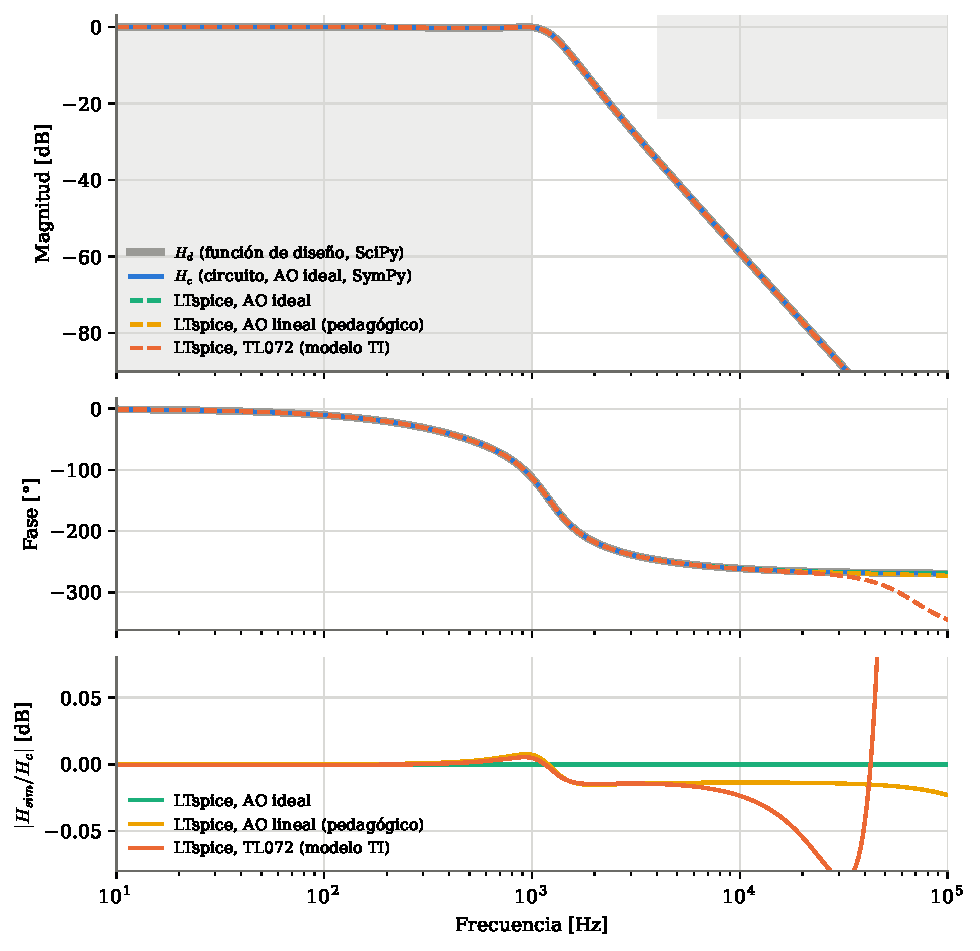
\includegraphics[width=0.92\linewidth]{fig_ltspice_ac}
  \caption{Respuesta en frecuencia: función de diseño, circuito ideal (SymPy) y simulaciones de LTspice. Abajo, diferencia de magnitud respecto de
  $H_c$ (la desviación del TL072 por encima de \qty{20}{\kilo\hertz} se analiza en la \cref{fig:ltspice_altafrec}).}
  \label{fig:ltspice_ac}
\end{figure}

\paragraph{Fuga en alta frecuencia.} Por encima de unos \qty{40}{\kilo\hertz}, el modelo del TL072 se aparta del circuito ideal
(\cref{fig:ltspice_altafrec}). A \qty{100}{\kilo\hertz} atenúa \qty{\vTLAcienk}{\decibel} en lugar de \qty{\vIdAcienk}{\decibel}, es decir,
\qty{\vTLdevCienk}{\decibel} menos. Es la limitación conocida del Sallen--Key de ganancia unitaria. A esas frecuencias $C_1$ y $C_2$ son casi
cortocircuitos, el nodo~4 queda unido a la salida y la corriente que entra por $R_1$ desde U1 se inyecta en la salida de U2. Con un AO real, la
impedancia de salida en lazo cerrado $Z_o \approx r_o/(1+A(j\omega))$ crece con la frecuencia y aparece un camino directo
$V_o \approx V_3\,Z_o/R_1$. Con $r_o \approx \qty{300}{\ohm}$ (macromodelo) y un GBW de \qty{3}{\mega\hertz}, esta estimación da
\qty{\vEstAcienk}{\decibel} a \qty{100}{\kilo\hertz}, del mismo orden que la simulación. El modelo lineal sin impedancia de salida no reproduce el
efecto. No compromete la plantilla, que exige \qty{24}{\decibel}, pero limita la atenuación última del filtro y debe tenerse en cuenta al medir la
banda de rechazo lejana.

\begin{figure}[H]
  \centering
  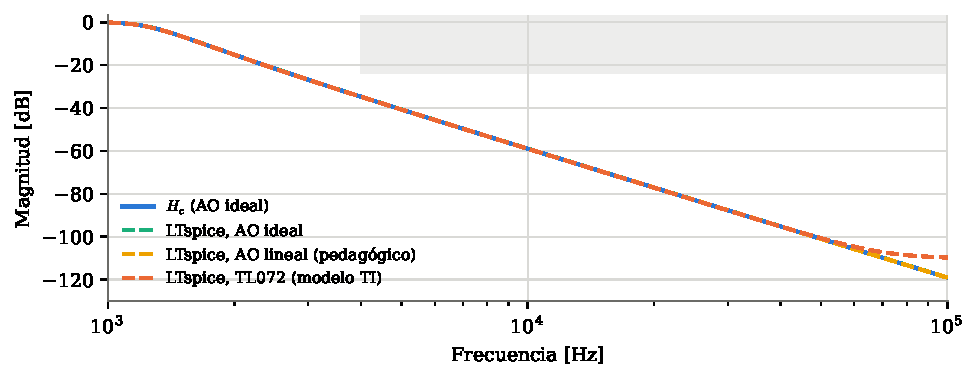
\includegraphics[width=0.85\linewidth]{fig_ltspice_altafrec}
  \caption{Banda de rechazo hasta \qty{100}{\kilo\hertz}: fuga del Sallen--Key de ganancia unitaria con el modelo del TL072.}
  \label{fig:ltspice_altafrec}
\end{figure}

\subsubsection{Transitorio senoidal}
Con una entrada senoidal de \qty{1}{\volt} eficaz a \qty{200}{\hertz}, \qty{1}{\kilo\hertz} y \qty{4}{\kilo\hertz} (\cref{fig:ltspice_tran}),
la ganancia y el desfase en régimen permanente se obtuvieron ajustando por mínimos cuadrados un seno de frecuencia conocida a la entrada y a la salida
entre \qty{20}{\milli\second} y \qty{30}{\milli\second}. Coinciden con $H_c(j\omega)$ dentro de \qty{0.02}{\decibel} y \ang{0.2}
(\cref{tab:ltspice_tran}). Las salidas de los AO no se acercan a la saturación.

\begin{figure}[H]
  \centering
  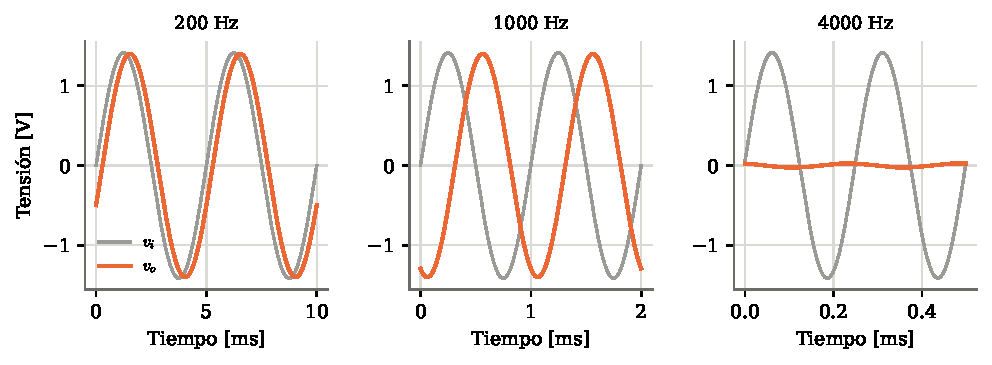
\includegraphics[width=\linewidth]{fig_ltspice_tran}
  \caption{Transitorio con el modelo del TL072: entrada y salida en régimen permanente (dos períodos).}
  \label{fig:ltspice_tran}
\end{figure}

\begin{table}[H]
  \centering\small
  \caption{Ganancia y fase obtenidas del transitorio de LTspice (TL072) frente a $H_c(j\omega)$.}
  \label{tab:ltspice_tran}
  \resizebox{\linewidth}{!}{\tabres{tab_ltspice_tran}}
\end{table}

\subsubsection{Respuesta al escalón}
Ante un escalón de \qty{1}{\volt}, la salida simulada con el TL072 sigue a la respuesta calculada de $H_c$ (\cref{fig:ltspice_escalon}). LTspice mide
un sobrepico de \qty{\vSobrepicoLT}{\percent}, frente a \qty{\vSobrepicoPy}{\percent} de $H_c$, con valor final \qty{1.000}{\volt}. En una primera
corrida se había obtenido \qty{9.99}{\percent}: LTspice comprime por defecto las formas de onda (\texttt{plotwinsize}) y había guardado solo 43
puntos, y las mediciones \texttt{.meas} se evalúan sobre esos datos comprimidos. Con \texttt{.options plotwinsize=0} se guardan los
\num{\vPuntosEscalon}~puntos calculados y la diferencia con el cálculo se reduce a centésimas de punto porcentual. Por eso todos los netlists de
transitorio incluyen esa opción.

\begin{figure}[H]
  \centering
  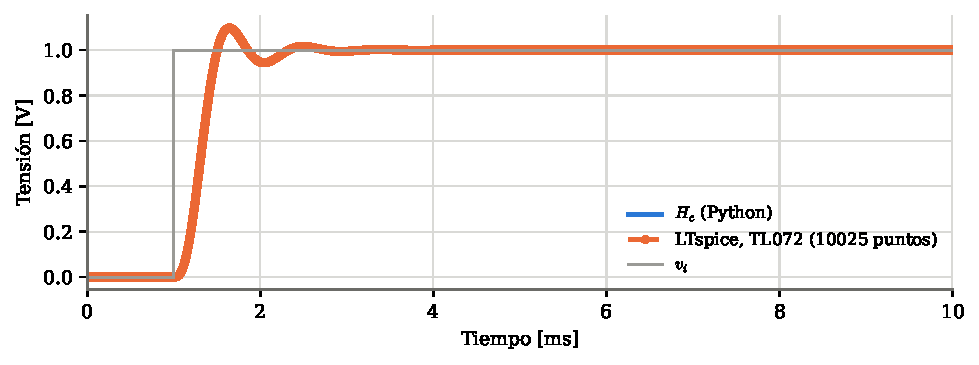
\includegraphics[width=0.9\linewidth]{fig_ltspice_escalon}
  \caption{Respuesta al escalón de \qty{1}{\volt}: $H_c$ (Python) y LTspice con el modelo del TL072.}
  \label{fig:ltspice_escalon}
\end{figure}

\subsubsection{Gran señal}
A \qty{936}{\hertz}, la frecuencia de mayor nivel interno, la salida alcanza \qty{\vGSmaxCuatro}{\volt} y \qty{\vGSmaxOcho}{\volt} de pico con
entradas de \qty{4}{\volt} y \qty{8}{\volt}, sin distorsión visible. Con \qty{11}{\volt} de pico recorta en \qty{\vGSmaxOnce}{\volt} y
\qty{\vGSminOnce}{\volt} (\cref{fig:ltspice_gran_senal}), mientras U1 llega solo a \qty{\vGSUunoOnce}{\volt} porque la etapa~1 ya atenúa a esa
frecuencia: la etapa que satura es U2. La excursión del modelo con \qty{\pm 12}{\volt} es de unos \qty{1.5}{\volt} por debajo de cada riel, de modo que
el límite de \qty{\pm 9}{\volt} adoptado en la \cref{sec:ao} es conservador y la amplitud propuesta para las mediciones (\qty{1}{\volt} eficaz)
tiene un margen de más de siete veces.

\begin{figure}[H]
  \centering
  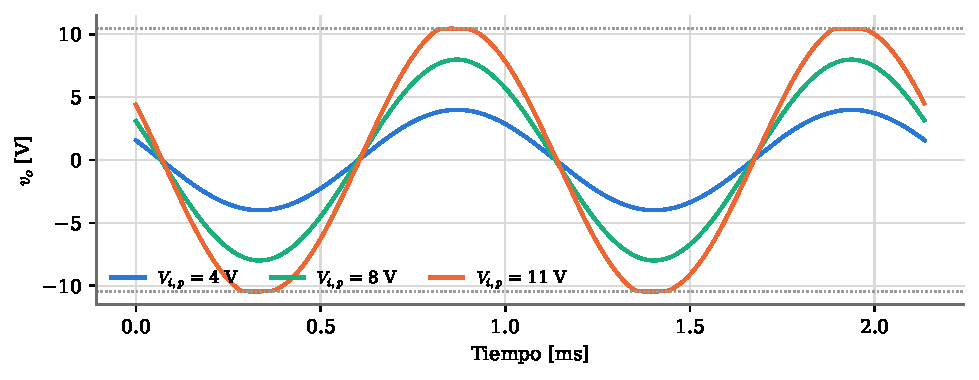
\includegraphics[width=0.9\linewidth]{fig_ltspice_gran_senal}
  \caption{Ensayo de gran señal a \qty{936}{\hertz} con el modelo del TL072 y alimentación de \qty{\pm 12}{\volt}.}
  \label{fig:ltspice_gran_senal}
\end{figure}
